\documentclass[12pt]{article}
\usepackage[scaled=0.8]{helvet}

%% the file should be rendered with pdflatex

%% THIS SECTION IS THE PREAMBLE
\usepackage{graphicx}
\usepackage[utf8]{inputenc}
\usepackage{tikz}
\usepackage{hyperref}
\usepackage{caption}
\usepackage{titlesec}
\usepackage{float}
\usepackage[formats]{listings}
\usetikzlibrary{shapes,arrows}
\usetikzlibrary{positioning}
\usepackage{fancyvrb}
\usepackage{soul}
\usepackage{lscape}
\usepackage{adjustbox}
\usepackage{amsmath}
\usepackage{booktabs}
\usepackage{tcolorbox}
\usepackage{enumitem}
\usepackage{babel}

\setcounter{tocdepth}{2}
\setlength{\abovecaptionskip}{25pt plus 3pt minus 2pt}

\newcommand{\mybox}[1]{%
\noindent
    \begin{tikzpicture}%
        \node[rectangle, draw=gray, fill = gray!10 , rounded corners=3pt, inner xsep=10pt, inner ysep=6pt, outer ysep=10pt]{
        \begin{minipage}{0.90\linewidth}#1\end{minipage}};%
    \end{tikzpicture}%
}

\newcommand{\Hint}[1]{%
\noindent
    \begin{tikzpicture}%
        \node[rectangle, draw=black, rounded corners=3pt, inner xsep=10pt, inner ysep=6pt, outer ysep=10pt]{
        \begin{minipage}{\linewidth}#1\end{minipage}};%
    \end{tikzpicture}%
}

\newcommand{\code}[1]{\texttt{#1}}
\newcommand{\oq}{``}
\newcommand{\cq}{''}

\begin{document}

  \begin{titlepage}
    \vspace*{\fill}
    \begin{center}

\begin{figure}
\centering
\includegraphics[scale=0.6]{Figures/ONDA_logo_v12.png}
\end{figure}

      {\Large \textbf{Good Practices for AI-Assisted Coding}}\\
      \vspace*{0.5\baselineskip}
      {\normalsize \textbf{O}pen methodologies for \textbf{N}eurorehabilitation and \textbf{D}ata \textbf{A}nalysis}\\
      \vspace*{1\baselineskip}
      \normalsize{Giorgio Arcara}\\
      \vspace*{3\baselineskip}
      {\normalsize version 0.1}\\
      \vspace*{1\baselineskip}
      \today
      \vspace*{2\baselineskip}

      \begin{minipage}{0.8\linewidth}
      \centering\small\itshape
      This document was drafted in collaboration with an AI language model (Claude, Anthropic).
      The ideas, structure, and editorial judgement are the author's own;
      the AI assisted with drafting, phrasing, and formatting.
      \end{minipage}
    \end{center}
    \vspace*{\fill}
  \end{titlepage}

\tableofcontents
\newpage

\thispagestyle{empty}
\vspace*{\fill}
\begin{figure}[H]
    \centering
    \includegraphics[width=0.65\textwidth]{Figures/AGC_chisafare.jpg}
    \caption*{\textit{``Chi sa fare, sa capire.''} --- Non è un proverbio. È la vita.}
\end{figure}
\vspace*{\fill}
\newpage


%% ─────────────────────────────────────────────
\section{Introduction}

Large Language Models (LLMs) such as ChatGPT, Claude, Copilot, and similar tools have become widely used aids in everyday coding tasks.
They are undeniably powerful: they can accelerate prototyping, suggest solutions to common problems, explain unfamiliar syntax, and reduce the time spent on boilerplate code.

In a research context, however, this efficiency comes with a risk that is easy to underestimate.

\subsection*{Your aim is framing correctly the problem}

In many professional contexts, code is the deliverable: if it works correctly and on time, the job is done.
Research is different. Code in research is a \emph{means}, not an end.
The real deliverable is framing and solving correctly a given problem, and the solution can only be as solid as the researcher's understanding of the pipeline that produced it.

Consider what it actually means to \emph{not} have a full understanding of your own analysis code:

\begin{itemize}
    \item You cannot defend your methodological choices, because you did not make them---you accepted them.
    \item You cannot catch errors before they become published mistakes. A bug that produces plausible-looking output is invisible to someone who does not know what the output \emph{should} look like.
    \item You cannot adapt the analysis to a new dataset, a reviewer's request, or a follow-up question, because you do not understand the logic well enough to modify it safely.
    \item You cannot teach or explain your methods to others, which undermines the very transparency that open science requires.
\end{itemize}

\noindent Working code produced without understanding is not a research output. It is a liability.
\pagebreak

\textbf{The understanding you build while writing the analysis is part of the scientific contribution itself}, not a side effect of it.
Velocity optimised at the cost of that understanding is a net loss, regardless of how clean the final script looks.

This guide does not argue against using LLMs. It argues for using them \emph{deliberately}.


%% ─────────────────────────────────────────────
\section{The Core Problem}

Learning to code---and to solve problems computationally---is a cognitive process that spans multiple levels of competence.
Bloom's Taxonomy, a well-established framework in educational psychology, describes six levels of cognitive skill, ordered from the most superficial to the most demanding:

\begin{figure}[H]
\centering
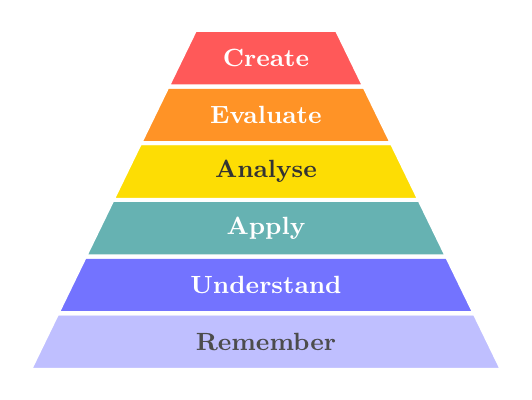
\begin{tikzpicture}[font=\small\bfseries]
  % Level 0: Remember (widest, at bottom)
  \filldraw[fill=blue!25, draw=white, line width=1.5pt]
    (-3.00,0.00) -- (3.00,0.00) -- (2.65,0.72) -- (-2.65,0.72) -- cycle;
  \node[black!70] at (0,0.36) {Remember};
  % Level 1: Understand
  \filldraw[fill=blue!55, draw=white, line width=1.5pt]
    (-2.65,0.72) -- (2.65,0.72) -- (2.30,1.44) -- (-2.30,1.44) -- cycle;
  \node[white] at (0,1.08) {Understand};
  % Level 2: Apply
  \filldraw[fill=teal!60, draw=white, line width=1.5pt]
    (-2.30,1.44) -- (2.30,1.44) -- (1.95,2.16) -- (-1.95,2.16) -- cycle;
  \node[white] at (0,1.80) {Apply};
  % Level 3: Analyse
  \filldraw[fill=yellow!80!orange, draw=white, line width=1.5pt]
    (-1.95,2.16) -- (1.95,2.16) -- (1.60,2.88) -- (-1.60,2.88) -- cycle;
  \node[black!80] at (0,2.52) {Analyse};
  % Level 4: Evaluate
  \filldraw[fill=orange!85, draw=white, line width=1.5pt]
    (-1.60,2.88) -- (1.60,2.88) -- (1.25,3.60) -- (-1.25,3.60) -- cycle;
  \node[white] at (0,3.24) {Evaluate};
  % Level 5: Create (narrowest, at top)
  \filldraw[fill=red!65, draw=white, line width=1.5pt]
    (-1.25,3.60) -- (1.25,3.60) -- (0.90,4.32) -- (-0.90,4.32) -- cycle;
  \node[white] at (0,3.96) {Create};
\end{tikzpicture}
\caption*{Bloom's Taxonomy of cognitive skills (bottom = most superficial, top = most demanding)}
\end{figure}

Genuine coding competence sits at the top: \textbf{Create}---the ability to design and produce solutions to novel problems.
Reaching it requires building through the intermediate levels: understanding why code behaves as it does, applying principles in unfamiliar contexts, analysing trade-offs, evaluating correctness.

LLMs disrupt this ladder. You don't create any working solution even if it may seem so. When a working solution is handed to you by LLM before you have wrestled with the problem, you interact with code at its lowest level---\textbf{Remember}: you recognise patterns, run scripts, adjust parameters, and produce outputs.
This is not competence. It produces the illusion of competence.

The risk differs depending on experience level:

\begin{itemize}
    \item \textbf{Experienced programmers} risk the gradual atrophy of higher-order skills---analysis, evaluation, design. The capacity to Create does not disappear overnight, but it quietly erodes as cognitive work is increasingly outsourced.
    \item \textbf{Junior researchers} risk becoming permanently anchored at Remember. Without ever climbing the intermediate levels of the taxonomy, there is no foundation on which genuine competence can develop. Familiarity with a codebase---running scripts, reading outputs---is not understanding it.
\end{itemize}

\begin{tcolorbox}[
    colback=red!5,
    colframe=red!70!black,
    boxrule=1pt,
    leftrule=4pt,
    arc=2pt,
    colbacktitle=red!70!black,
    title={\textbf{Key Principle}},
    fonttitle=\bfseries\color{white}
]
All good practices described in this guide share one goal: \textbf{pushing you up Bloom's Taxonomy}---away from the passive familiarity that LLMs enable, and toward the active competence that research demands.
\end{tcolorbox}


%% ─────────────────────────────────────────────
\section{Define the Problem First}

Before any of the practices in the following sections can help, there is a prerequisite step that applies to everyone, regardless of experience level: \textbf{define the problem before you open the editor---or the LLM.}

In research, coding exists to solve a problem. That sounds obvious, but it has a non-obvious implication: if the problem is not clearly defined, no amount of working code solves it. An LLM is very good at solving the problem you give it---the risk is giving it the wrong problem because you have not thought it through yourself first.

Defining the problem means being able to answer, in plain language, \emph{before} writing a single line:

\begin{itemize}
    \item What question am I trying to answer?
    \item What does the input look like, and what should the output look like?
    \item What would a correct result look like, and how would I recognise a wrong one?
\end{itemize}

\noindent If you cannot answer these questions, you are not ready to code---and you are certainly not ready to prompt.
This step is not a practice to add to a checklist: it is the foundation that makes every other practice meaningful.

%% ─────────────────────────────────────────────
\section{Practices for Experienced Programmers}

If you already have solid programming experience, the primary risk is not that you will fail to understand LLM output---it is that you will stop \emph{bothering} to.
The practices below are designed to keep your problem-solving muscle active.

\subsection{Trace before you accept}

Before accepting any non-trivial block of LLM-generated code, trace through it mentally (or with pen and paper). Ask yourself:
\begin{itemize}
    \item What does each step do?
    \item What are the edge cases or failure modes?
    \item Would I have written it differently, and why?
\end{itemize}
If you cannot answer these questions, do not commit the code.

\subsection{Design the algorithm first}

For any problem that requires more than a few lines of logic, sketch the algorithm yourself before prompting. Use pseudocode, a diagram, or plain English. Then use the LLM to \emph{implement} your design, not to invent it.
\pagebreak

\mybox{
\textbf{Pattern to avoid:} \emph{``Here is my data. Write me a function that does X.''}\\[4pt]
\textbf{Pattern to prefer:} \emph{``I want to loop over rows, filter by condition Y, and aggregate using Z. Help me implement this.''}
}

\subsection{Periodically code without LLM assistance}

Schedule regular sessions---even short ones---where you work entirely without LLM assistance. These serve as a diagnostic: if a task you once found easy now feels surprisingly difficult, that is a signal worth taking seriously.

\subsection{Seek friction deliberately}

Efficiency is not always the goal. When learning a new library, domain, or language, resist the temptation to let the LLM smooth every bump. Struggle is the mechanism of learning.


%% ─────────────────────────────────────────────
\section{Practices for Junior Researchers}

If you are early in your programming journey, the risk is subtler and more insidious: you can develop \emph{operational fluency}---the ability to run, modify, and talk about code---without a corresponding mental model.
The practices below are self-directed and do not require a mentor.

\subsection{Blank-page reconstruction}

After receiving and using a piece of LLM-generated code, close it. Then try to rewrite it from scratch without looking. Do not aim for perfection---aim for understanding.
Where you get stuck reveals exactly what you have not yet understood.

\subsection{Inverted rubber duck}

The classical \oq rubber duck debugging\cq{} technique involves explaining your code out loud to force clarity.
The \emph{inverted} version: explain the LLM's code back to the LLM in your own words, then ask it to identify any gaps or errors in your explanation.

\begin{tcolorbox}[
    colback=blue!5,
    colframe=blue!40!black,
    boxrule=1pt,
    leftrule=4pt,
    arc=2pt,
    colbacktitle=blue!40!black,
    title={\textbf{Example prompt}},
    fonttitle=\bfseries\color{white}
]
\emph{``Here is my understanding of what this function does: [your explanation]. Are there any steps I have described incorrectly or any important aspects I have missed?''}
\end{tcolorbox}

\subsection{Write tests before asking for code}

Before asking the LLM to write a function, write down (in plain language or actual test cases) what correct behaviour looks like: given this input, what should the output be?
This forces you to understand the problem before you receive the solution.

\subsection{Keep a bug journal}

Keep a running log of bugs you have encountered and how they were resolved. Focus on the \emph{why}: what was your incorrect mental model, and how did it get corrected?
Over time, this journal becomes a record of your understanding growing.

\subsection{Change one variable at a time when debugging}

When something does not work, resist the temptation to ask the LLM to fix it immediately. Debugging is precisely where you practise the higher levels of Bloom's Taxonomy---Analyse and Evaluate---and those levels cannot be climbed by delegation. Form a hypothesis about what is wrong, change exactly one thing, and observe the result. Only reach for the LLM after you have made at least one genuine attempt to diagnose the problem yourself.

\subsection{Decompose the problem yourself before prompting}

For any non-trivial task, write down the sub-problems before opening the LLM. This does not need to be formal---a rough bullet list is enough. The act of decomposition is where much of the learning happens, and it is precisely what gets skipped when you prompt immediately.


%% ─────────────────────────────────────────────
\section{Quick Reference}
\footnotesize
\begin{center}
\begin{tabular}{p{0.44\textwidth} p{0.44\textwidth}}
\toprule
\multicolumn{2}{c}{\textbf{Everyone: define the problem before coding or prompting}} \\
\midrule
\textbf{Experienced programmers} & \textbf{Junior researchers} \\
\midrule
Trace all LLM code before accepting & Blank-page reconstruction after using LLM code \\
\addlinespace
Design the algorithm before prompting & Inverted rubber duck (explain code back, ask for gaps) \\
\addlinespace
Code without LLM regularly (diagnostic) & Write test cases before asking for code \\
\addlinespace
Seek friction deliberately when learning & Keep a bug journal (focus on the \emph{why}) \\
\addlinespace
 & Change one variable at a time when debugging \\
\addlinespace
 & Decompose the problem yourself before prompting \\
\bottomrule
\end{tabular}
\end{center}

\vspace{1em}
\normalsize

\mybox{
\textbf{Shared principle for both groups:} \emph{Use the LLM to implement and to check, but not to think in your place}.
The goal is not to avoid LLMs. The goal is to remain the author of your own understanding.
}


\end{document}
